\documentclass{jarticle}
\usepackage{lmodern}
\usepackage{twocolumn}
%\usepackage[dvi ps]{graphicx}%%画像を読み込む
\usepackage[dvipdfmx]{graphicx}
\usepackage{subfigure}
\usepackage{amsmath}          %%genfrac http://www.biwako.shiga-u.ac.jp/sensei/kumazawa/tex/form006.html
\usepackage{ulem}             %%http://biwako.shiga-u.ac.jp/sensei/kumazawa/tex/ulem.html     uline,uuline,uwave,sout,xoutなど
\usepackage{multirow}
\usepackage{here}
%\usepackage{setspace}
\usepackage{chukan2020}       %%最後に読み込むこと!(最後に読み込まないと\textwidthなどの設定が反映されない)

\pagestyle{empty} %ページ番号を入れるときにはコメントアウトする

\begin{document}

\linesparpage{50}

\title{
改良型細径空圧筋を用いたカニ模倣型ロボットの開発
}
\etitle{
Development of Crab-type Robot Using an Improved Thin Pneumatic Mustle
}
\author{
\centering
研究者 濱口 紘生  指導教員 中西 大輔
}
\eauthor{
Keywords: McKibben Pneumatic Actuater, Exoskeleton, Biomimetic Robot
}

\maketitle

\thispagestyle{empty}  %1ページ目にページ番号を入れるときにはコメントアウトする

%%%%%%%%%%%%%%%%%%%%%%%%%%%%%%%%%%%%%%%%%%%%%%%%%%%%%%%%%%%%%%%%%%%%%%%%%%%%%%%
\section{緒言}

代表的な人工筋肉として,圧縮空気を印加することにより骨格筋のように収縮するMcKibben型人工筋肉(MPA)があげられる.
従来は直径が数十mm程度のものが多かったが,近年では数mm程度のMPAが注目を集めている\cite{wakimoto}.
その細さを活かして小さい筋肉,あるいは集積によって複雑な筋肉を表現可能なことから,筋骨格系ロボットに盛んに用いられている\cite{wakimoto}.
一方で,甲殻類のような外骨格を有する生物模倣ロボットでは,アクチュエータの配置が困難なことからワイヤ駆動や関節にサーボモータを配置したものが主流であった\cite{crabrobot1}.
細径MPAであれば骨格内部にアクチュエータを配置することが可能であり,実際の生物に近い構成でロボットを作成することが可能である.そこで本研究では外骨格生物のうち甲殻類の蟹をモデルに,
実際の蟹の筋肉と関節の構造を参考にして細径MPAを使用した蟹の歩脚ロボットの開発に取り組む.

%%%%%%%%%%%%%%%%%%%%%%%%%%%%%%%%%%%%%%%%%%%%%%%%%%%%%%%%%%%%%%%%%%%%%%%%%%%%%%%
%\vspace*{-2mm}
\section{細径MPAを用いた羽状筋の再現}
%\vspace*{-1mm}
羽状筋とは,筋肉全体が斜めの角度で腱に付着する筋肉形状を指し,同じ断面積内に多くの筋繊維を収めることが可能であることから高い力を発生する特性を有する.
本研究では,先行研究\cite{crabrobot2}で開発された細径MPAを用いた羽状筋の課題解決に取り組んだ.

まず制作方法について,本研究では端部部品を改良し、ゴムと端部を接着剤で,スリーブと端部をOリングと接着剤でそれぞれ固定する方式へと変更した.(図\ref{fig:OringMPA}下)
これにより細径MPAの作成に練度が不要となり,作製時間が大幅に短縮された.

続いて細径MPAの収縮性能向上に取り組んだ.
細径MPAに用いるスリーブに対して事前に熱加工を行うことで折癖をとるとともにスリーブの初期直径を2 mmにまで小さくすることに成功した.
これにより0.6 MPa印加時の収縮率が16 %から20 %まで向上させることができた.

最後に細径MPAを羽状配置するために端部の部品ん構造を改良した.
羽状筋は収縮した際に筋肉の角度(羽状角)が変化するが,先行研究\cite{crabrobot2}では根元の角度が固定されており,腱の引き込みの妨げになっていた.
そこで本研究では図\ref{fig:MPAparts}に示すように細径MPA端部部品に自由度を持たせた.
図\ref{fig:MPAparts}中,赤斜線部の穴に回転軸が左右からはまる構造になっている.
これにより,細径MPAが収縮して腱が引き込まれた際にも羽状角が変化することが可能となった.
%%%%%%%%%%%%%%%%%%%%%%%%%%%%%%%%%%%%%%%%%%%%%%%%%%%%%%%%%%%%%%%%%%%%%%%%%%%%%%%
%\begin{figure}[H]
%  \begin{minipage}[b]{0.47\columnwidth}
%    \centering
%    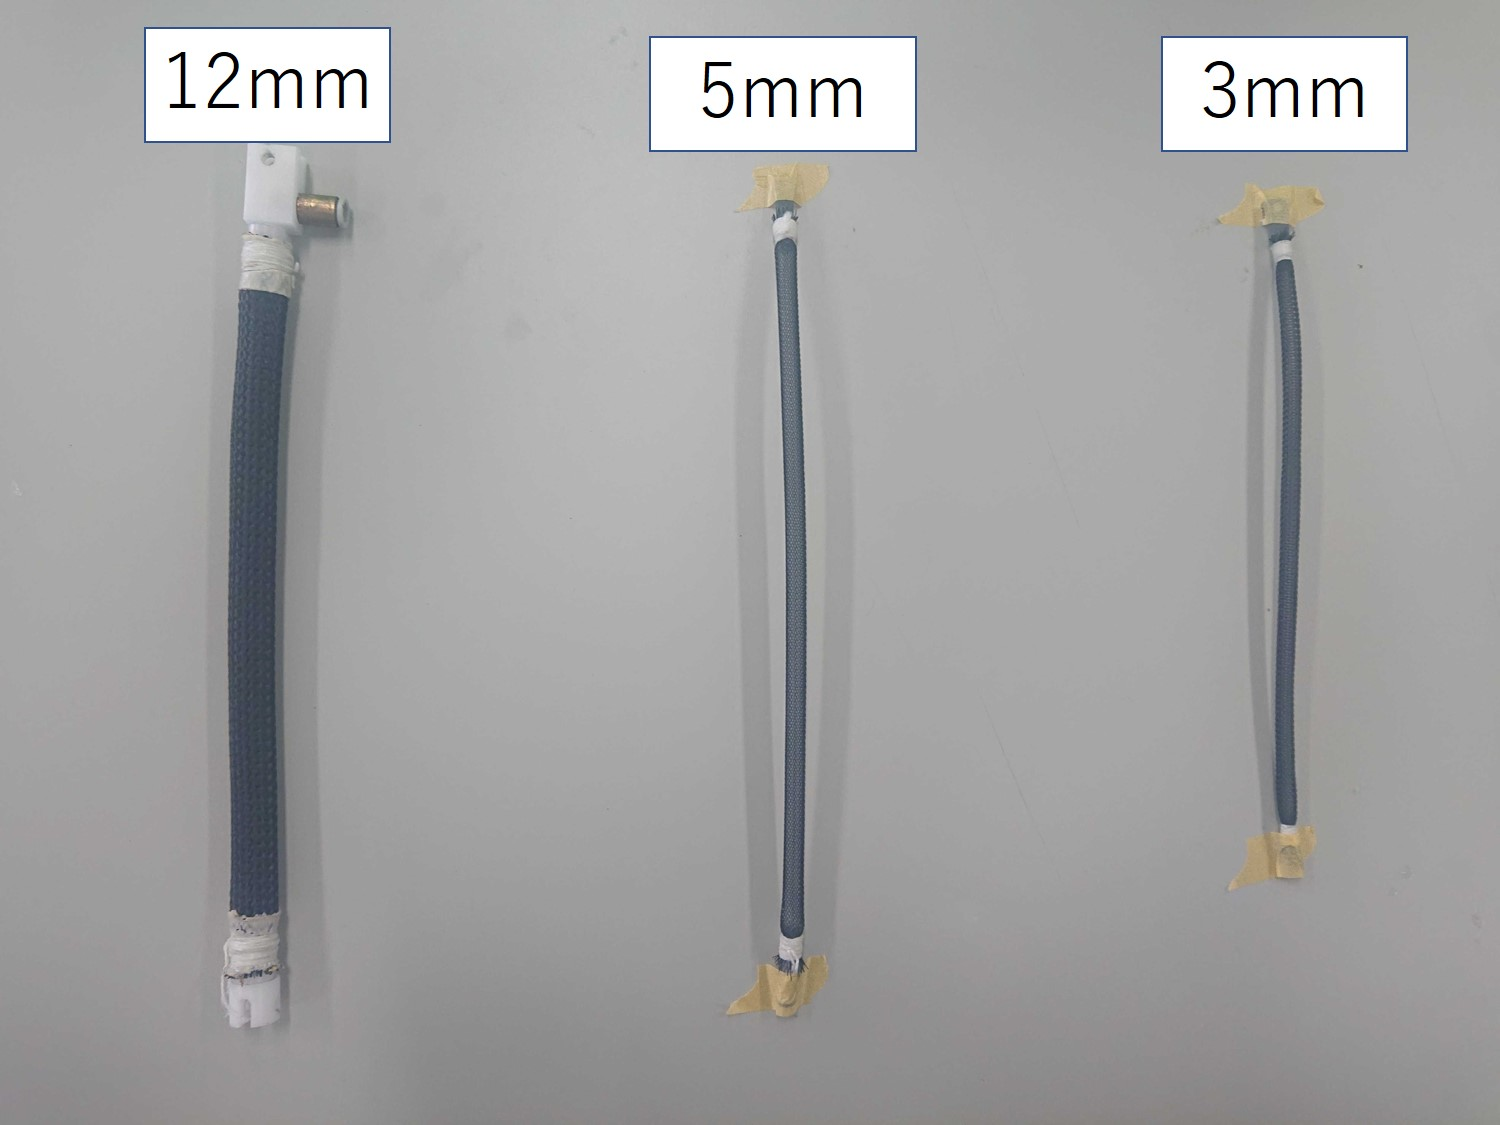
\includegraphics[scale=0.13]{image/mpa.JPG}
%    \vspace{-4mm}
%    \caption{MPAの外径}
%    \label{fig:MPA}
%  \end{minipage}
%  \hspace{0.04\columnwidth}
%  \begin{minipage}[b]{0.47\columnwidth}
%    \centering
%    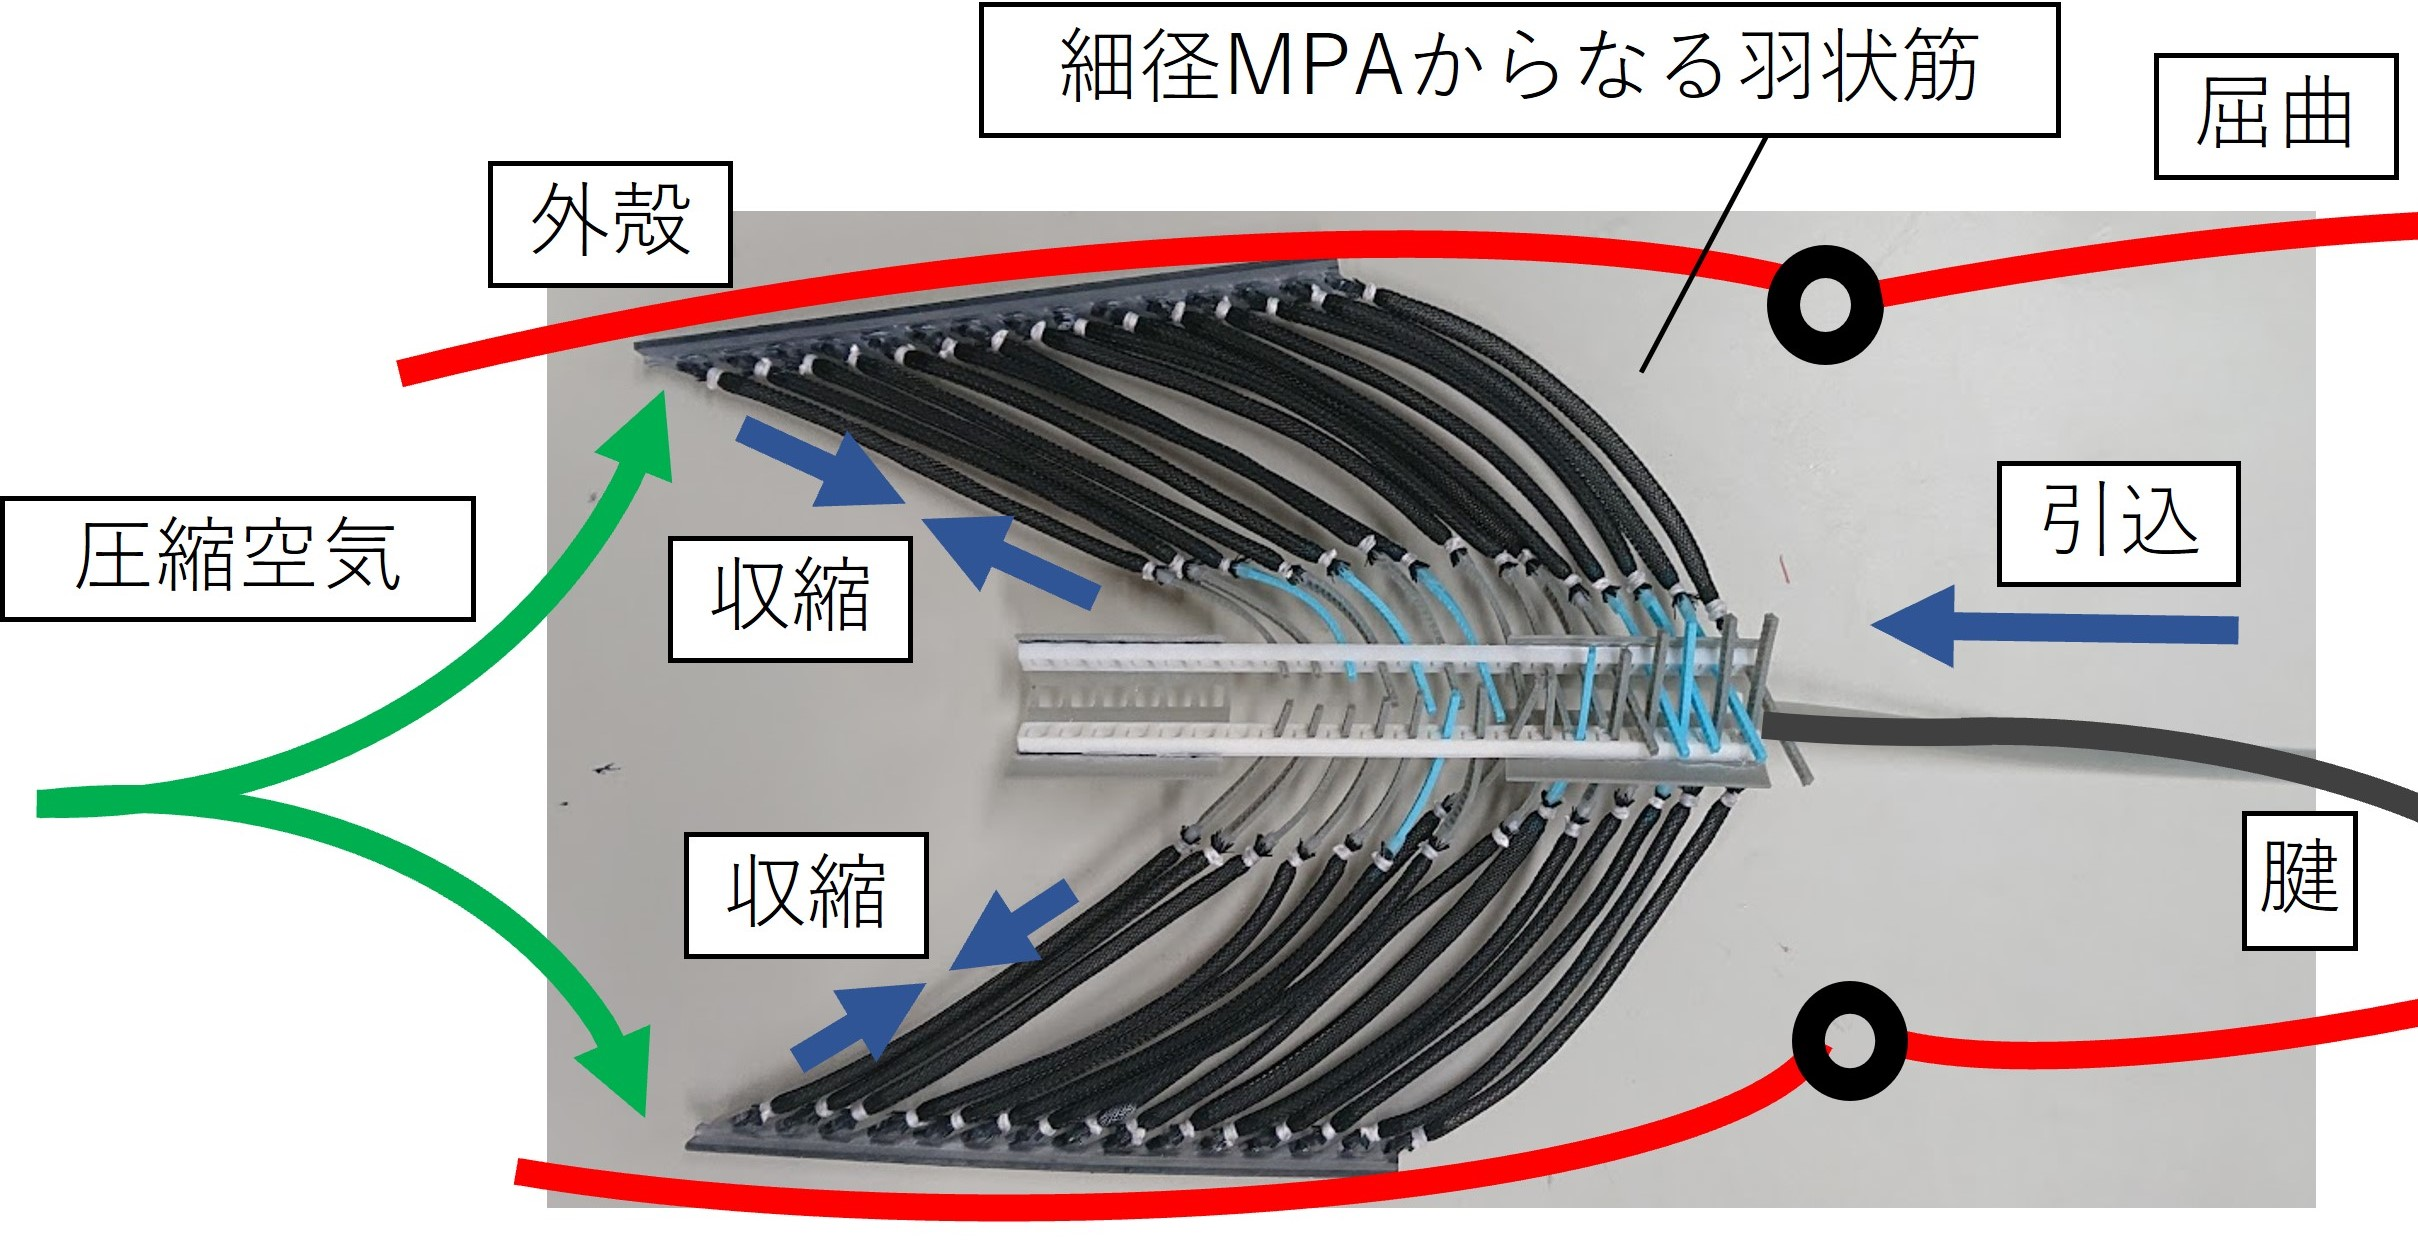
\includegraphics[scale=0.19]{image/mosiki.JPG}
%    \vspace{-6mm}
%    \caption{蟹模倣ロボット\cite{crabrobot2}}
%    \label{fig:crabrobot}
%  \end{minipage}
%\end{figure}
%\vspace*{-5mm}
\begin{figure}[!t]
  \begin{minipage}[b]{0.4\columnwidth}
    \centering
    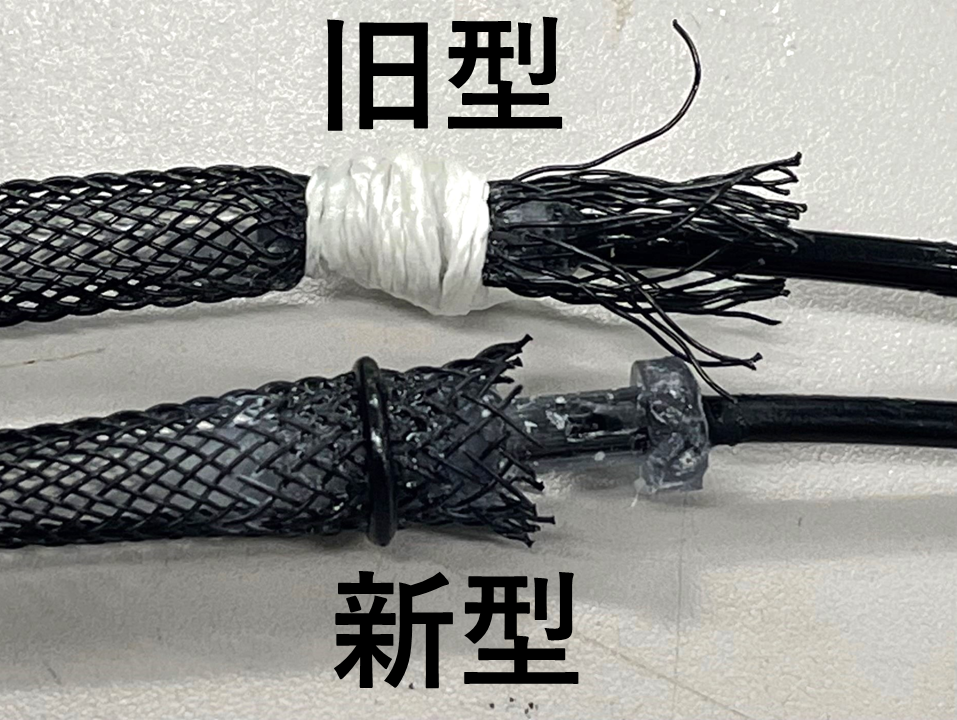
\includegraphics[scale=0.115]{image/hikaku.png}
    \vspace{-6mm}
    \caption{MPA締結方法}
    \label{fig:OringMPA}
  \end{minipage}
  \begin{minipage}[b]{0.54\columnwidth}
    \centering
    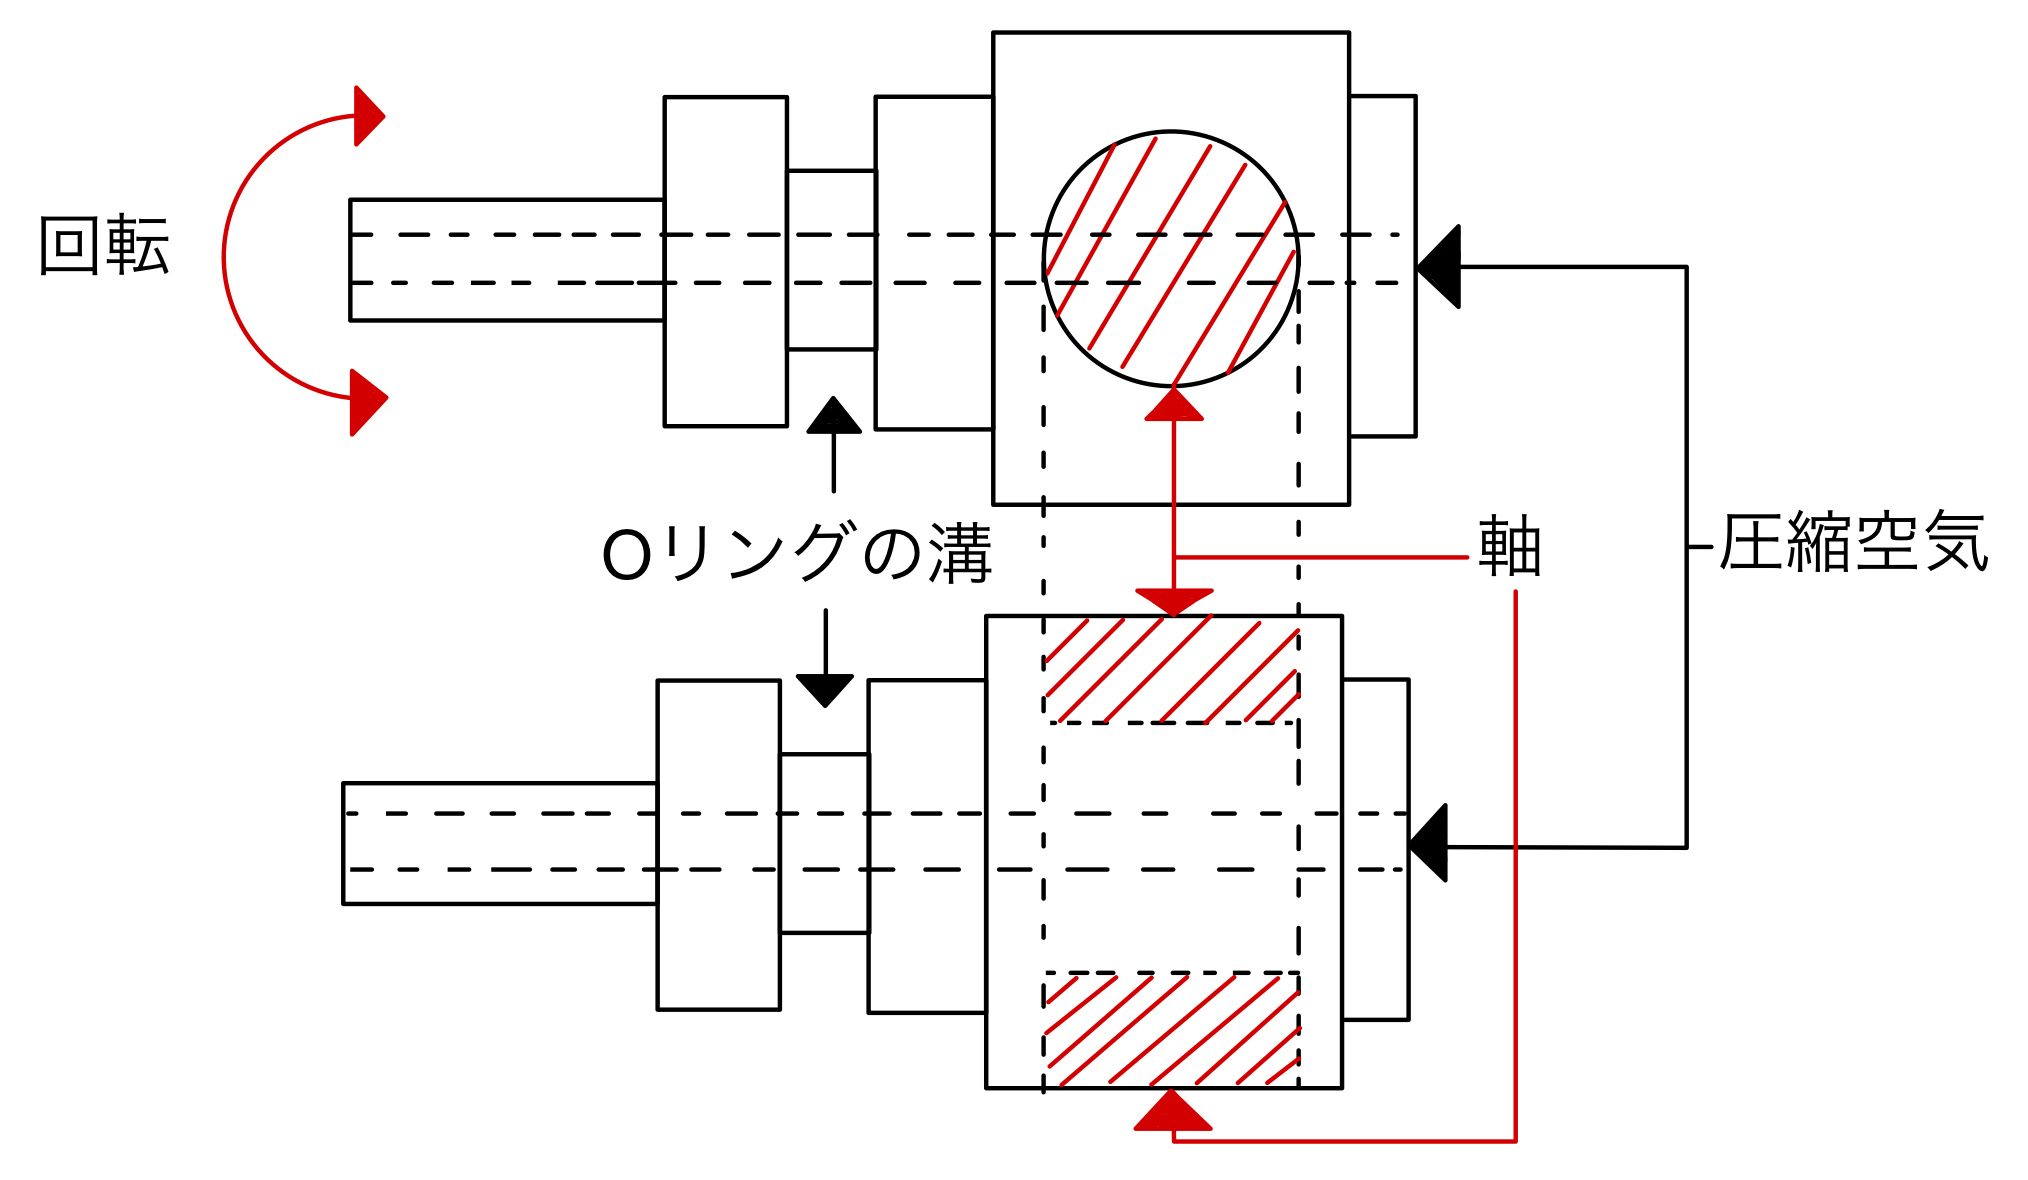
\includegraphics[scale=0.056]{image/MPA_irast.jpg}
    \vspace{-8mm}
    \caption{細径MPA部品}
    \label{fig:MPAparts}
  \end{minipage}
\end{figure}
%%%%%%%%%%%%%%%%%%%%%%%%%%%%%%%%%%%%%%%%%%%%%%%%%%%%%%%%%%%%%%%%%%%%%%%%%%%%%%%
\begin{figure}[t]
  \centering
  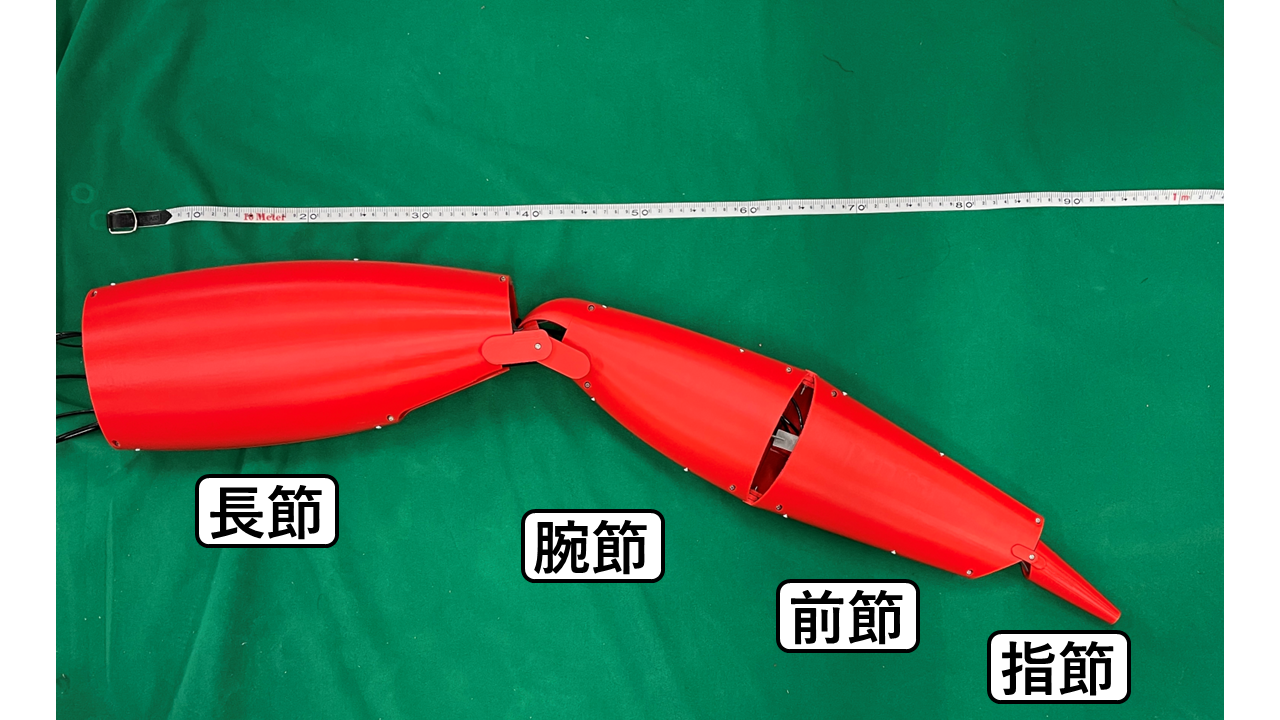
\includegraphics[scale=0.15]{image/jikki.png}
  \vspace{-2mm}
  \caption{実機の外観}
  \label{fig:jikki}
\end{figure}
%%%%%%%%%%%%%%%%%%%%%%%%%%%%%%%%%%%%%%%%%%%%%%%%%%%%%%%%%%%%%%%%%%%%%%%%%%%%%%%
\begin{figure}[t!]
    \centering
    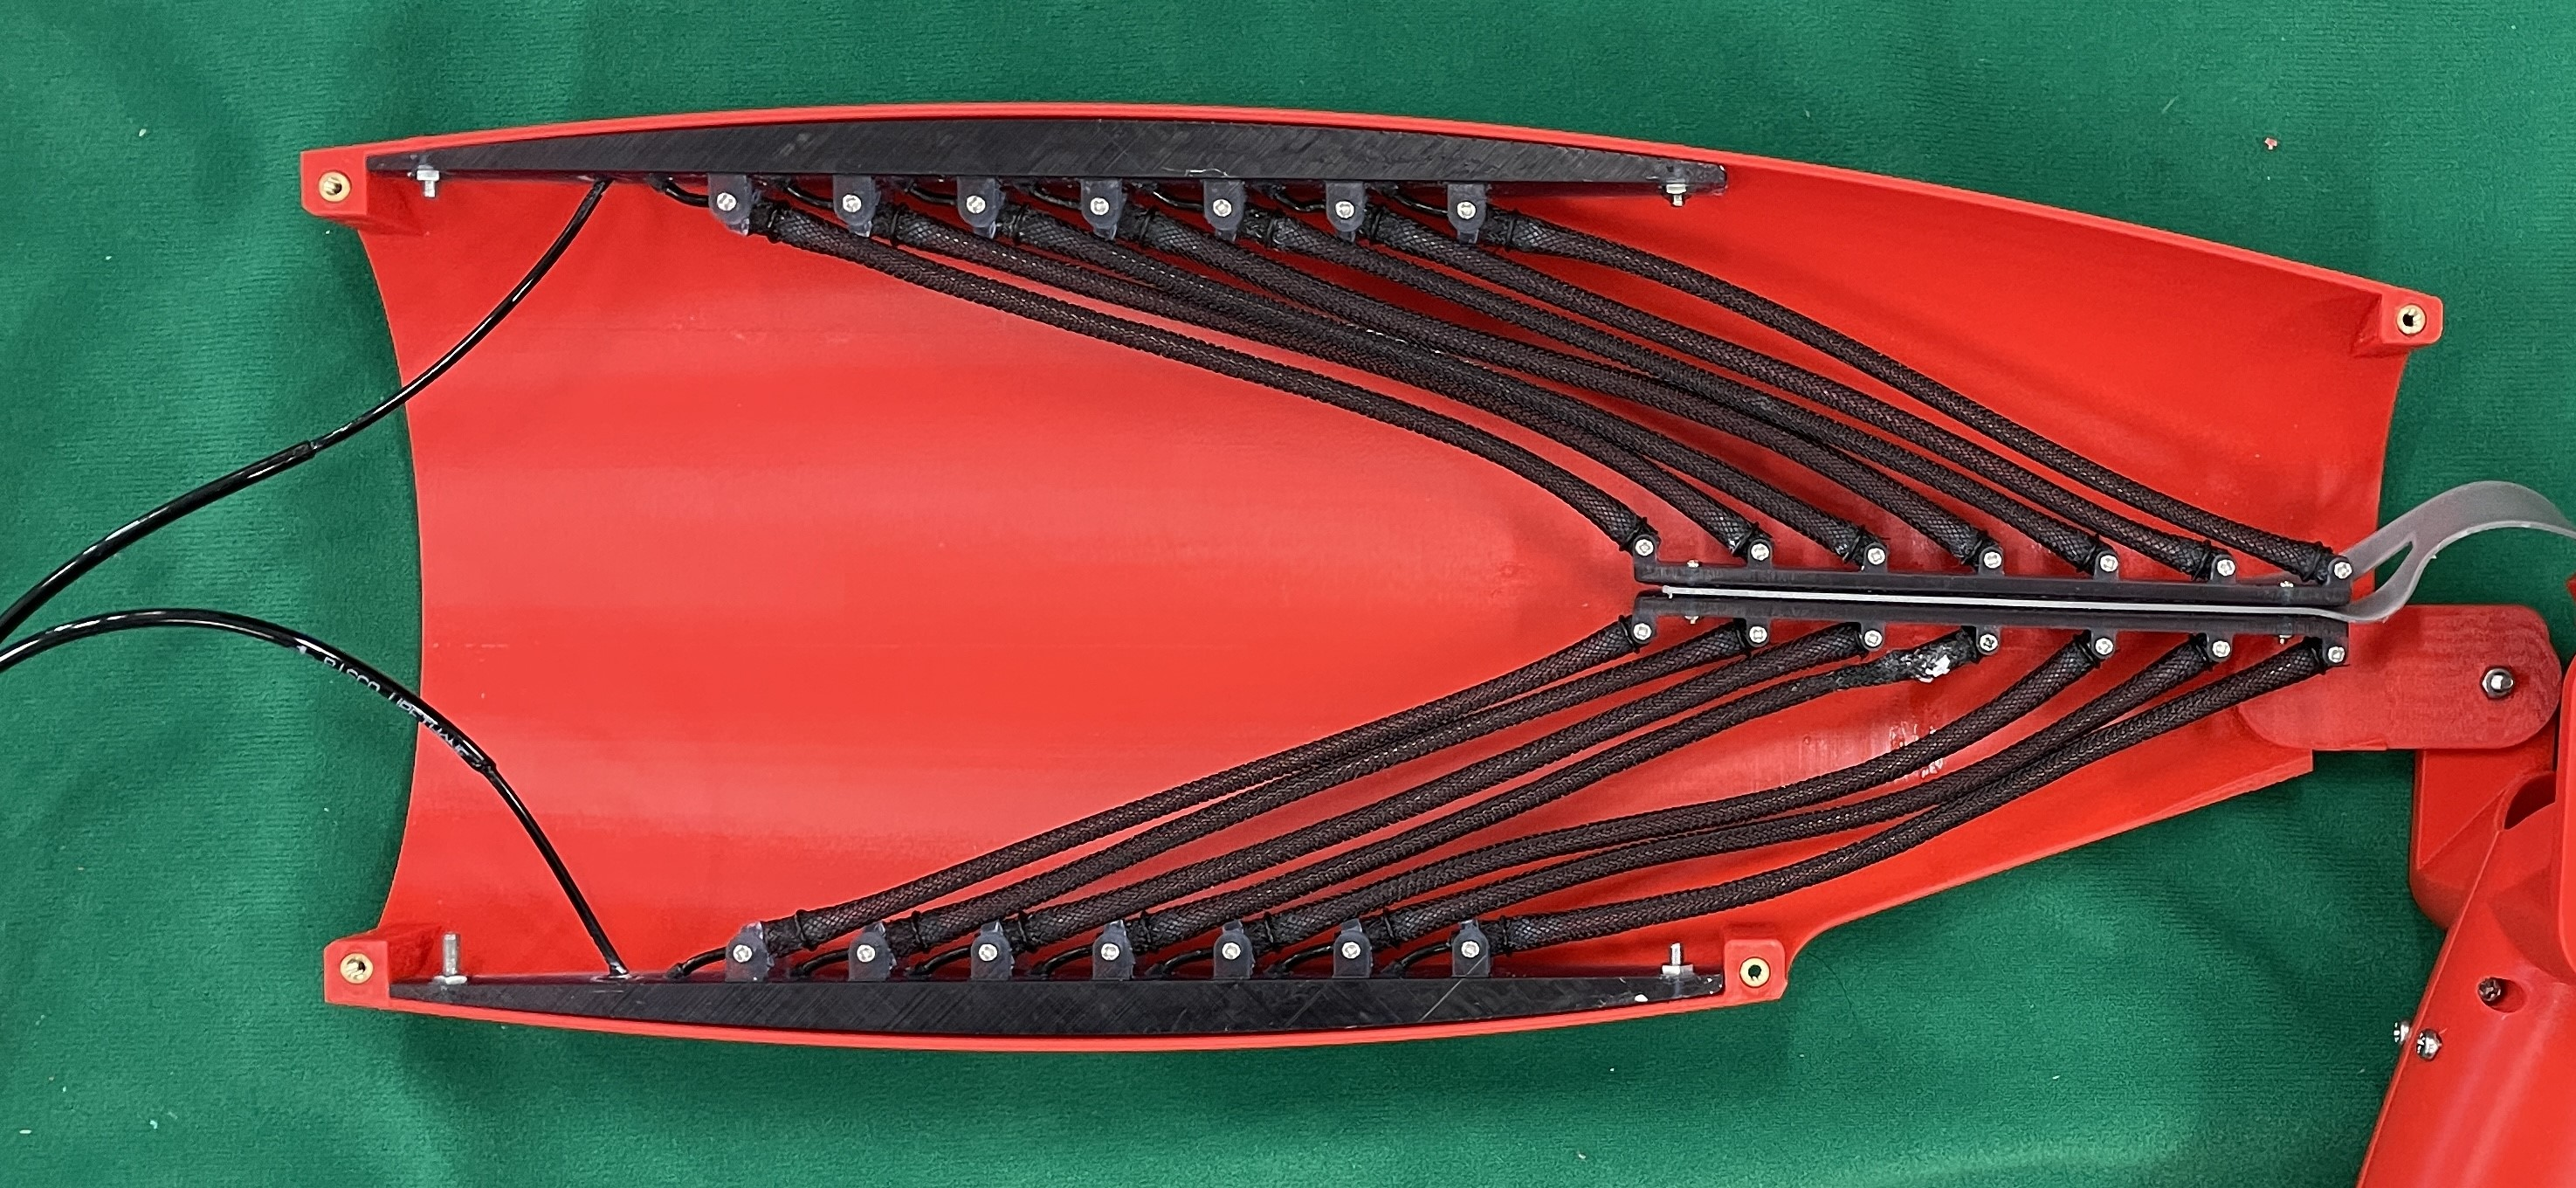
\includegraphics[scale=0.05]{image/crabmuscle.jpg}
    \vspace{-4mm}
    \caption{実機の筋配置}
    \label{fig:muscle}
\end{figure}
%%%%%%%%%%%%%%%%%%%%%%%%%%%%%%%%%%%%%%%%%%%%%%%%%%%%%%%%%%%%%%%%%%%%%%%%%%%%%%%
\begin{table}[t]
  \centering
  \vspace{-2mm}
  \caption{実際の蟹と実機の可動域比較}
  \vspace{1mm}
  \scalebox{0.8}{ 
      \begin{tabular}{|c|c|c|c|}
          \hline
          項目/可動域[deg] & 長節-腕節間 & 腕節-前節間 & 前節-指節間 \\ \hline
          実際の蟹 & 52$\sim$130 & 0$\sim$45 & 0$\sim$89 \\ \hline
          計算上のロボト & 41.7$\sim$127.97 & 0$\sim$27 & 0$\sim$32.35 \\ \hline
          実際のロボット & 45.3$\sim$133.1 & 3.25$\sim$36.0 & 9.82$\sim$39.8 \\ \hline
      \end{tabular}
  }
  \label{tab:kadouiki}
\end{table}
%%%%%%%%%%%%%%%%%%%%%%%%%%%%%%%%%%%%%%%%%%%%%%%%%%%%%%%%%%%%%%%%%%%%%%%%%%%%%%%
%\vspace{-4mm}
\begin{figure}[t]
  \centering
  \subfigure[長節-腕節間の動作実験]{
  \label{fig:move1} 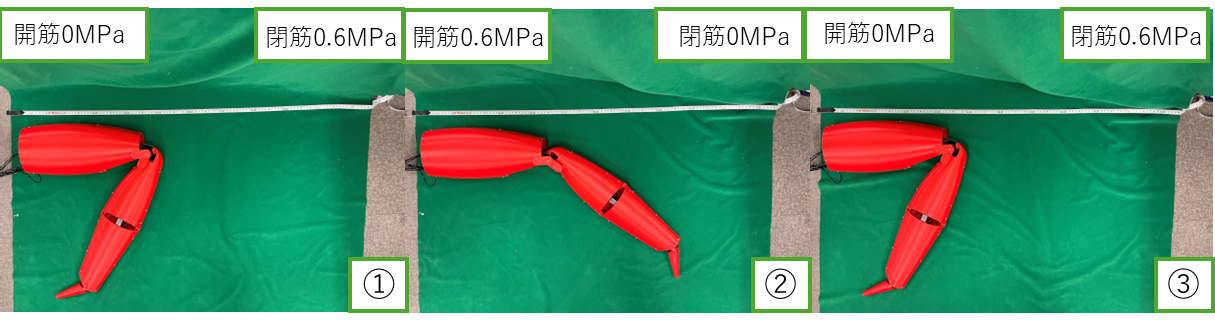
\includegraphics[scale=0.23]{image/chousetu-wansetu_edited.png}}
  \vspace{-2mm}
  \centering
  \subfigure[腕節‐前節間の動作実験]{
  \label{fig:move2} 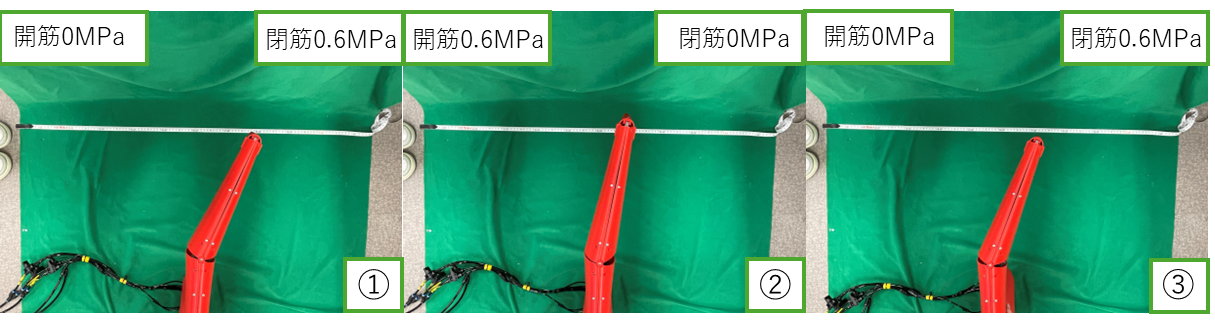
\includegraphics[scale=0.23]{image/wansetu-zensetu_edited.png}}
  \vspace{-2mm}
  \centering
  \subfigure[前節‐指節間の動作実験]{
  \label{fig:move3} 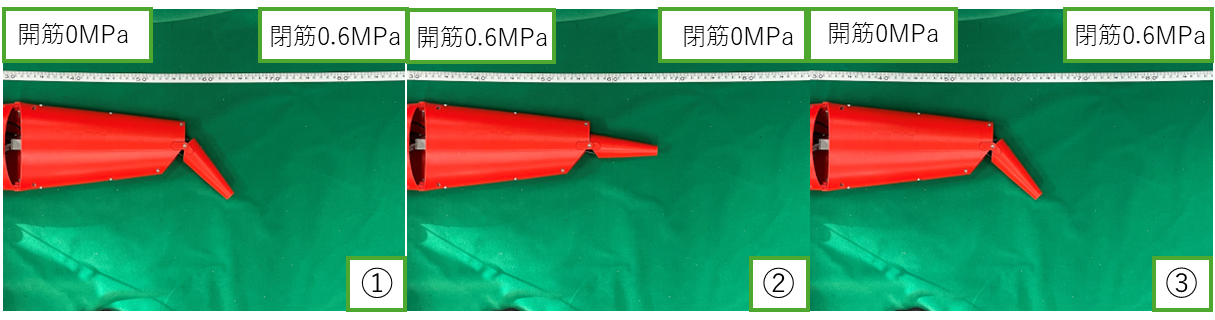
\includegraphics[scale=0.23]{image/zensetu-sisetu_edited.png}}
  \vspace{-2mm}
  \caption{動作実験の様子}
  \label{fig:jikken}
  \vspace{-2mm}
\end{figure}

%%%%%%%%%%%%%%%%%%%%%%%%%%%%%%%%%%%%%%%%%%%%%%%%%%%%%%%%%%%%%%%%%%%%%%%%%%%%%%%
%\vspace*{2mm}
\section{実機の設計・作成方法}
%\vspace*{-1mm}
%\subsection{外骨格の設計について}

作成した実機を図\ref{fig:jikki}に示す.
今回の研究では甲殻類のうち蟹のズワイガニの歩脚モデルに機体を作成した.
機体作成時には先行研究\cite{crabrobot2}のズワイガニの歩脚の各部寸法と,本研究で新たに解剖した際に得られた可動域をもとにしてモデリングした.
ただし機体内部に細径MPAや腱部品などを配置する必要があるため,実測値に対して直径方向には7倍,長手方向には3.5 倍のサイズとした.
しかし,上記のサイズ変更では腕節部の外骨格内部へアクチュエータの配置が困難であったため,長手方向のみを5.2倍に変更した.
作成にはFDM方式の3Dプリンタを使用し,関節部にはベアリングを入れている.
長手方向の具体的な寸法としては,長節が350 mm,腕節が256 mm,前節が245 mm,指節が100 mmである.
%%%%%%%%%%%%%%%%%%%%%%%%%%%%%%%%%%%%%%%%%%%%%%%%%%%%%%%%%%%%%%%%%%%%%%%%%%%%%%%
%\vspace{-1mm}
%\subsection{細径MPAを用いた羽状筋の再現方法}

開発した羽状筋を図\ref{fig:muscle}に示す.
上記で説明した実際の蟹の羽状筋の筋繊維は1本ずつ長さが異なっているが,開発のしやすさを優先して,図\ref{fig:muscle}のように細径MPAの長さがすべて等しくなるように設計した.
図\ref{fig:muscle}の細径MPAの端部は2章で紹介した細径MPAの収縮に合わせて羽状角が変化できる部品である.この部品は光造形方式の3Dプリンターで作製した.
また図\ref{fig:muscle}にある灰色の部品は蟹の腱を模したもので,TPU素材を使用してFDM方式の3Dプリンターで作製したので柔軟性が高い.
腱と外骨格は全てねじで固定しており,腱の張り具合は調整可能な仕組みになっている.

表\ref{tab:kadouiki}にカニの各関節の可動域を計測した結果を示す.
またロボットにおいては,この可動域が再現できるように腱の付着位置などを設計した.
計算上の各関節の可動域を表\ref{tab:kadouiki}に示す.
ここで腕節-前節間と前節-指節間については実際の可動域よりも設計上の可動域のほうが狭いが,これは今回の「全ての細径MPAの長さは等しい」という設計方針では可動域の再現が不可能であるためである.
より広い可動域を実現するためには,短い筋や関節の再現が必要であるが,今後の課題とする.
%%%%%%%%%%%%%%%%%%%%%%%%%%%%%%%%%%%%%%%%%%%%%%%%%%%%%%%%%%%%%%%%%%%%%%%%%%%%%%%
%\begin{eqnarray}
%	\label{theta2} \theta_2 &=& \sin^{-1}\left(\frac{d}{0.8 \ell_1}\right)\\
%  \label{Se} S_e &=& \ell_1 \cos\theta_1 - \ell_2 \cos\theta_2
%\end{eqnarray}

%%%%%%%%%%%%%%%%%%%%%%%%%%%%%%%%%%%%%%%%%%%%%%%%%%%%%%%%%%%%%%%%%%%%%%%%%%%%%%%
%\vspace*{-2mm}
\section{動作実験}
関節の動きを確認しやすくするために長節-腕節間と前節-指節間は機体を寝かせた状態,腕節-前節間は機体を立てた状態で動作実験を行った.
また,初期位置は開筋か閉筋のどちらか一方が張った状態の位置にし,圧縮空気の印加は手動で行い印加圧力は0.6MPa,開筋と閉筋の手動弁を交互に開閉することで動作させた.
ここで開筋は関節を開く方向に,閉筋は閉じる方向に作用する羽状筋を指す.

長節-腕節間の動作結果を図\ref{fig:move1},腕節-前節の動作実験を図\ref{fig:move2},前節-指節の動作実験を図\ref{fig:move3}に示す.
結果より,長節-腕節間では初期状態(図\ref{fig:move1}左)と最終状態(図\ref{fig:move1}右)では歩脚の角度が近い状態になった.
腕節-前節間,前節-指節間では長節-腕節間と同じような動きがみられたが,可動域が少し狭く感じられた.

そこでトラッキングソフト(kinovia)を用いて動作時の関節可動域を計算した(表\ref{tab:kadouiki}).
その結果,長節腕節間では実際の蟹の可動域を再現できていることを確認した,腕節-前節間では設計通りの可動域が再現できていることを確認した,前節-指節間では設計通り可動域が再現できていることを確認した.
%%%%%%%%%%%%%%%%%%%%%%%%%%%%%%%%%%%%%%%%%%%%%%%%%%%%%%%%%%%%%%%%%%%%%%%%%%%%%%%
%\vspace*{-5mm}
%\section{考察}

計算した可動域との差が出た原因について考察する.
原因として,腱の固定方法が挙げられる.図\ref{fig:kenkotei},図\ref{fig:ken_moshiki}に本研究で作製した実機の腱固定方法を示す.
本研究では腱をねじで押さえつけて固定する方法を採用した.
しかし,この固定方法では腱をどれほどの長さで固定すればいいかがわからなくなってしまう.
それにより計算上の腱の長さと差が生じ,圧力を印加していない状態で張力が発生してしまい可動域にも差が生じてしまったと考えられる.
そのため,ロードセルを用いて張力が発生しないように腱を固定する必要があると考えた.
もう1つの原因として,可動域を計算する際に使用した簡易モデルが挙げられる.
本研究では実機のおおよその可動域を計算するために実機の簡易モデルを用いたが,その簡易モデルでは細径MPAを腱に固定する部品の高さを考慮していなかった.
これにより計算上の細径MPAのストロークと差が出てしまい,簡易モデルと実機との間で可動域の差が出てしまったと考えられる.
この問題を解決するために実機に近い構造を持つモデルを構築し,それを用いてより正確な可動域を計算する必要があると考えた.
%%%%%%%%%%%%%%%%%%%%%%%%%%%%%%%%%%%%%%%%%%%%%%%%%%%%%%%%%%%%%%%%%%%%%%%%%%%%%%%
\begin{figure}[t]
  \begin{minipage}[b]{0.47\columnwidth}
    \centering
    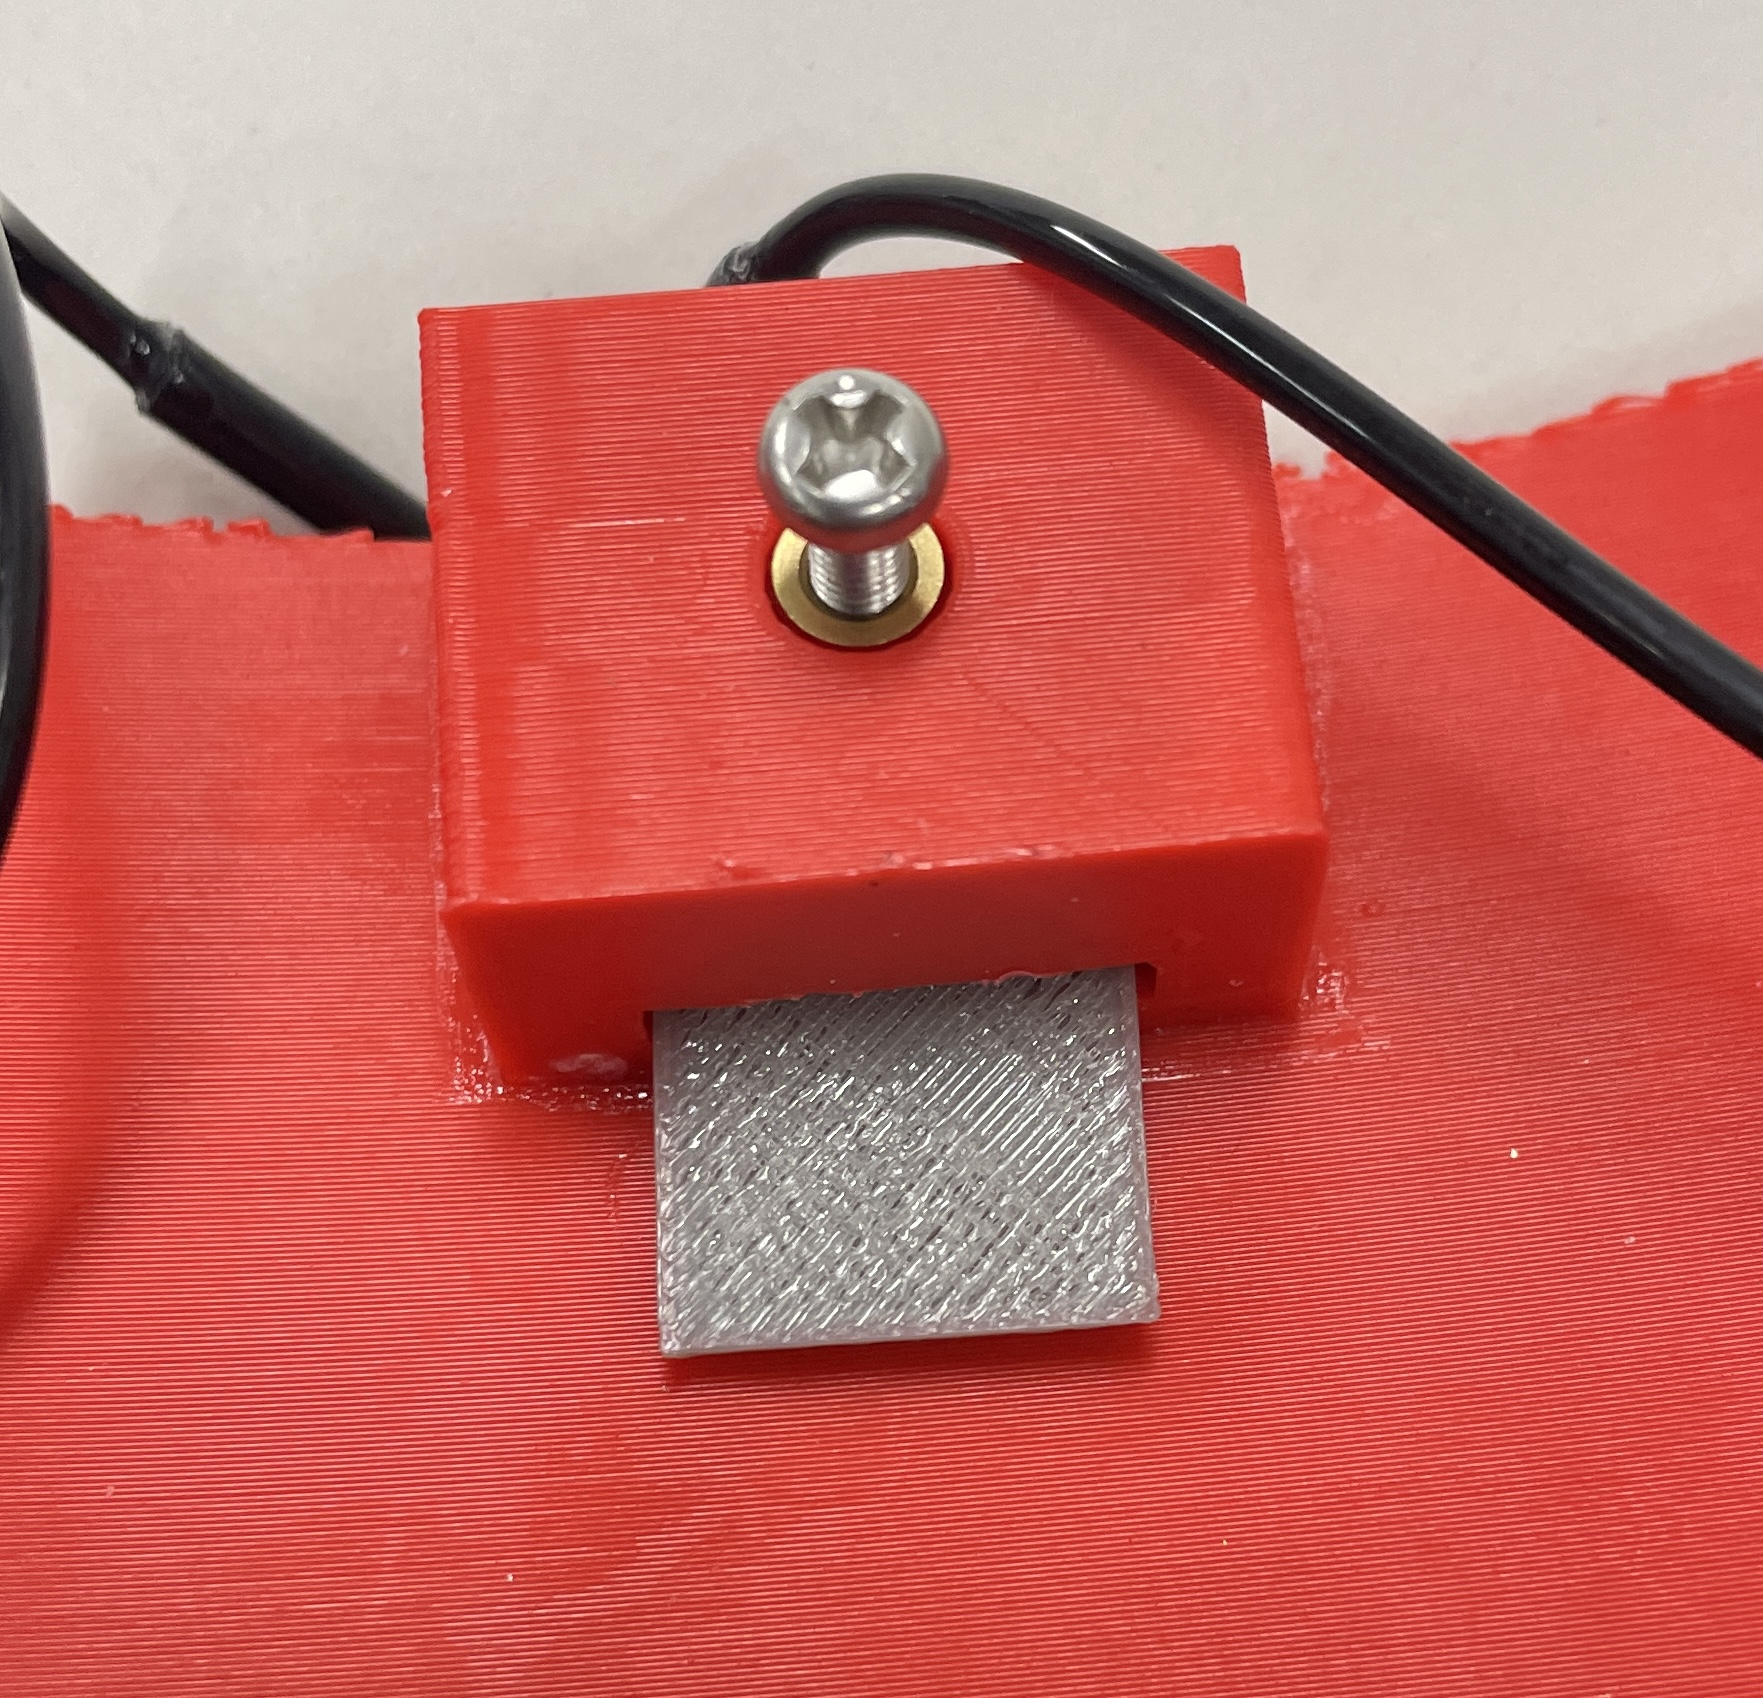
\includegraphics[scale=0.17]{image/kenkotei.jpg}
    \vspace{-2mm}
    \caption{腱の固定方法}
    \label{fig:kenkotei}
  \end{minipage}
  \hspace{0.04\columnwidth}
  \begin{minipage}[b]{0.47\columnwidth}
    \centering
    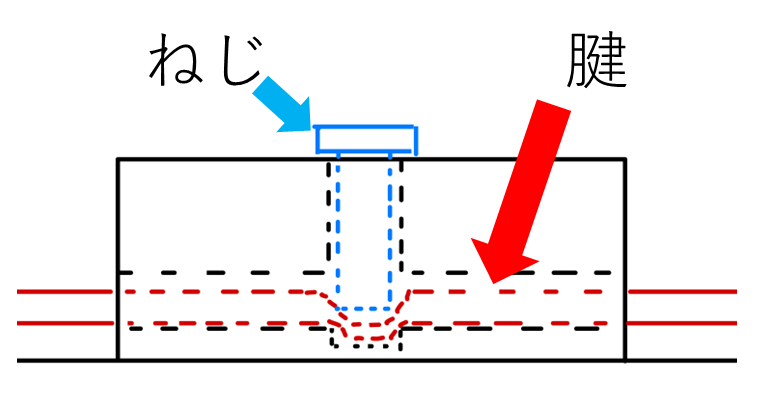
\includegraphics[scale=0.17]{image/moshiki_edited.png}
    \vspace{1mm}
    \caption{腱固定方法の模式図}
    \label{fig:ken_moshiki}
  \end{minipage}
\end{figure}
%%%%%%%%%%%%%%%%%%%%%%%%%%%%%%%%%%%%%%%%%%%%%%%%%%%%%%%%%%%%%%%%%%%%%%%%%%%%%%%
%\vspace*{-2mm}
\section{結言}
本稿では,外骨格生物模倣ロボットの開発をするにあたって課題となる細径MPA の作成方法と固定方法について改良を行った.
さらにそれらを用いてカニ模倣型ロボットの開発に成功し,長節から指節までの動作実験を行った.
節の開閉動作を確認することができ,計算上の可動域に近い動作を確認することができた.
今後は多様な長さの細径MPAを配置する方法,細径MPAに圧縮空気を印加していない状態で張力が発生しない固定方法を考えることにより実際の蟹の動きに近づけるような歩脚ロボットの完成を予定している.
%%%%%%%%%%%%%%%%%%%%%%%%%%%%%%%%%%%%%%%%%%%%%%%%%%%%%%%%%%%%%%%%%%%%%%%%%%%%%%%
\begin{thebibliography}{99}
  \bibitem{wakimoto}
  脇本修一,
  細径McKibben型人工筋の開発と用途開拓,
  計測と制御,57巻,11号,pp.812-815,2018
  
  \bibitem{crabrobot1}
  CHEN, Xi, et al. Study on the Design and Experimental Research on a Bionic Crab Robot with Amphibious Multi-Modal Movement, Journal of Marine Science and Engineering,10,12,p.1804,2022
  
  \bibitem{crabrobot2}
  中西大輔,長谷川侑大,浪花啓右,杉本靖博,
  細径空圧筋を用いた羽状筋および外骨格生物模倣ロボットの開発,ロボティクス・メカトロニクス講演会2024,2A1-L08,2024.

  \bibitem{crab}
  D.Hazerli and S.Richter,
  Why“swimming crabs”are able to swim-The importance of the axial skeleton:A comparison between the“swimming crab”Liocarcinus depurator and two other brachyuran crabs (Cancer pagurus, Carcinus maenas) using μCT and 3D-reconstruction,
  Arthropod Structure&Development,
  59,p.100972,2022

 \end{thebibliography}
 %%%%%%%%%%%%%%%%%%%%%%%%%%%%%%%%%%%%%%%%%%%%%%%%%%%%%%%%%%%%%%%%%%%%%%%%%%%%%%%
\end{document}